\documentclass[onecolumn, 10pt]{aastex63}
\usepackage{graphicx}%Include figure files
\usepackage[normalem]{ulem}
\usepackage{ulem}
% easy way to highlight new stuff
\newcommand{\new}[1]{{\color{blue} #1}}
\newcommand{\question}[1]{{\color{red} #1}}
\newcommand{\eg}{\emph{e.g.}}
\newcommand{\ie}{\emph{i.e.}}
\newcommand{\opsim}{\texttt{OpSim}}

\begin{document}

\title{How do we prepare to discover the unknown}

\correspondingauthor{Federica Bianco}
\email{fbianco@udel.edu}

\author{Fabio }
\affiliation{Department of , University of }

\author{Xiaolong }
\affiliation{Department of Physics and Astronomy, University of Delaware, Newark, DE 19716-2570, USA}

\author{Federica Bianco}
\affiliation{Department of Physics and Astronomy, University of Delaware, Newark, DE 19716-2570, USA}
\author{Will Clarkson}
\affiliation{University or Michigan - Dearborn}

\date{\today}

\begin{abstract}
The Rubin Observatory Legacy Survey of Space and Time
%Large Synoptic Survey Telescope 
(LSST) should open up new regions of parameter space for objects that move or otherwise vary.
%, with its unique survey capability,  will %have the potential to make unexpected %discoveries. 
The survey is expected to start in 2023 and facilities and data reduction pipelines are being finalized. The design of the facility, as well as the overall observing strategy, are
%overall observing strategy is designed, 
driven by the four core science themes of investigating dark matter and energy, exploring the transient and variable universe, mapping the Milky Way, and producing a catalog the Solar System objects from Near Earth Objects to the outer Solar System of unprecedented completeness. Yet perhaps the most exciting promise of the LSST is the prospect to discover phenomena and objects never seen before or even predicted from theory: \question{unknown-unknowns}. But in finalizing the details of the observing strategy, how can we assure that strategy decision will maximize our ability to discover unknown phenomena?  An observing strategy consists of sets of observational choices: pointings in the sky, alternation of filters, cadence of observations in the same field. Rubin LSST strategy proposals are evaluated by metrics under the Metric Analysis Framework (MAF) API. Although many metrics have been designed to assess how well a proposed strategy would discover planets, or exploding stars, and allow us to extract their physical properties, designing a metric to evaluate LSST's ability to discover unknown phenomena is a conceptually and practically challenging task that no one had yet attempted.
We create a Rubin LSST metric for \question{unknown-unknowns} by mapping planned LSST observations to a phase space defined by the brightness, color, and the change of those features and exploring the completeness in this phase space, and considering the extent of the proposed survey footprint,  and the ability to identify anomalously moving objects and structures. We measure the ability of 75 currently simulated \new{surveys}~to discover anomalies  including anomalies in color, lightcurve evolution, association, and proper motion. Our results allows  Rubin Observatory to design a survey that maximizes our chances to discover unknown unknowns.
\end{abstract}

\keywords{LSST, transients, proper motion, survey design}


\section{Introduction} \label{sec:intro}

The Rubin Observatory Legacy Survey of Space and Time (LSST hereafter), expected to begin in 2023, is an ambitious project that promises to monitor the entire southern hemisphere sky with high sensitivity, high {(seeing-limited) spatial} resolution, and high temporal cadence (
$\geq$ 1 image per night,  $\sim$ few days repeat on each field). While other surveys have stretched into one or two directions in these feature space, delivering high cadence observation on small fields of view for example (such as SNLS: \citealt{snls}) or large field of view monitoring at low resolution (like ASAS-SN: \citealt{asas-sn}), {the combination of} high spatial resolution, high cadence, and high sensitivity, places the Rubin LSST  in a unique position to contribute to nearly all fields of astronomy with an unprecedentedly rich data-set. Yet perhaps the most exciting promise of the Rubin LSST is its potential to discover as-yet unknown phenomena. This work focuses on assessing the potential of LSST to discover ``unknown-unknowns'': phenomena that have neither been observed, nor predicted, under different strategic observing choices. 
The Rubin LSST observing strategy is designed to accomplish several science goals within four science themes: (1) Probing dark energy and dark matter.
(2) Taking an inventory of the solar system.
(3) Exploring the transient optical sky.
(4) Mapping the Milky Way. These diverse goals lead to strict interlocking constraints including requirements on image quality, depth --- single visit depth and number of visits per field --- filters system, and total sky coverage. Detailed description of the science drivers and technical requirements can be found in \citet{lsst}.\footnote{For the Science Requirements Document (SRD) itself, see \citet{lsstSRD}.} Nonetheless, these constraints still allow for a significant flexibility in the details of the observing strategy. For example: while the reference design \citep[e.g.][]{designSystem, designCamera} leads to a revisit time of 3 days on average for 
$10,000 ~\mathrm{deg}^2$ of sky, with two visits per night, this allows for a large range of distributions and even median values for the inter-night time gaps in observations that are still possible while satisfying this requirement, as seen in Figure \ref{fig:tgaps_example}. {Additionally, there will be many ``surveys'' within the Legacy Survey of Space and Time: the majority of the 10 years will be spent on a survey designed explicitly to meet the requirement specified in \cite{designSystem}: the ``Wide-Fast-Deep'' survey. It is expected that this will take between 75\% and 85\% of the time on-sky. The remaining time will be spent on ``special programs'', incuding ``minisurveys'' (special coverage of extended areas of sky), ``Deep-Drilling-Fields'' (single pointings that will be visited periodically at an enhanced cadence and to reach a higher cumulative depth in the stacked images), and potentially ``Targets of Opportunity'' follow up of multi-messenger triggers.}

% WIC 2020-06-22 I found the description of the simulations, the opsims, the mafs, cosep, whitepapers, and metrics & FoMs to be a little bit compressed and hard to follow. Here's my attempt to give just a bit more context. 
{Perhaps uniquely among modern surveys, the Rubin Observatory Project team has shared its extensive simulations framework with the scientific community at a very high level of detail, including (but not limited to): detailed hardware specifications, facility operations models (including overheads at a high level of detail), atmospheric transmission, and astrophysical populations \citep{simsFramework}. For most users in the scientific community, it is the metadata of the predicted observing strategies (e.g. observing time, expected seeing, instantaneous depth to $5\sigma$~photometric precision) that is most relevant to evaluation of survey strategies: the project has made available to the community a large number (well over two hundred to-date) runs from its Operations Simulator \citep{opsim}, which generates the metadata for a full ten-year period of operation under specified desiderata for the run characteristics (for brevity, in this paper we refer to a simulated 10-year survey as an \opsim. Led by Lynne Jones \& Peter Yoachim at the University of Washington, the project has also developed a dedicated Metrics Analysis Framework (\texttt{MAF}: \citealt{maf})\footnote{Also available at \url{https://www.lsst.org/content/lsst-metrics-analysis-framework-maf}}, and continues to work with the community in the development of the tools to extract the scientific utility of the \texttt{OpSims} for various scientific cases. Standard metrics run on all \texttt{OpSims} by the project fall under the main \texttt{sims\_maf} package,\footnote{\url{https://github.com/lsst/sims_maf}} while community-contributed metrics are curated at the \texttt{maf-contrib} project.\footnote{\url{https://github.com/LSST-nonproject/sims_maf_contrib}}. We discuss the Operations Simulator and \texttt{MAF} in a little more detail in Section \ref{sec:MAF}.}

{Recent community input on the LSST survey strategy roughly divides into three phases. The first phase concluded with the development of the ``Community Observing Strategy Evaluation Paper'' (COSEP; \citealt{cosep}), which attempted to distill the requirements of a wide range of science cases into specifications (and in some cases evaluations) of simple quantitative measures of scientific effectiveness that could be compared between science cases. In the second phase,  the community was asked by the project to prepare cadence whitepapers to suggest alternatives to the baseline cadence; 46 whitepapers were ultimately submitted.\footnote{\url{https://www.lsst.org/submitted-whitepaper-2018}} In the current phase, the community is working to implement the quantitative scoring for the various science cases to allow them to be compared on a timescale commensurate with the ultimate decisions by the project on the survey strategy to adopt. This paper forms part of this third phase of community input.}

{A word on notation is in order. Following the naming convention of the the COSEP, we will used the acronym ``MAF'' (or sometimes the term ``metric'') to refer to a piece of code that measures properties of an \opsim~ on a per-field basis. The overall evaluation of a strategy requires assessing its power over a large number of scientific goals. Therefore, in order to be useful for comparison, the \texttt{MAF}s must be summarized themselves into Figures of Merit (FoMs): single numbers that convey the power of a survey (as simulated) to achieve a specific science goal. An example of a {\it metric} might be a characterization of the time-gaps between repeat observations of each field in a particular filter-pair of interest, while the associated$FoM$ would collapse the distribution into a single number that captures the sensitivity of the strategy to the detection of transients in some range of parameter space. For more on the operational definitions of metrics and FoMs, see the COSEP \citep{cosep}. }

%A number of simulated LSST surveys have been produced by the Rubin Data Management (?) team \citep{simsFramework} reflecting different requirements as proposed by the scientific community in a series of white paper.\footnote{\url{https://www.lsst.org/submitted-whitepaper-2018}. } Survey simulations are generated through the Operations Simulation (\opsim~ \citealt{opsim}) framework, and can be evaluated within the Metric Analysis Framework (\texttt{MAF}: \citealt{maf})\footnote{Also available at \url{https://www.lsst.org/content/lsst-metrics-analysis-framework-maf}}. Hereafter,  \new{following the naming convention of the COSEP, we will used the acronym ``MAF'' or as well ``metric'' to refer to a piece of code that measures properties of an \opsim~: the map of evaluated quantities on a field-by-field basis. The figure of merit (FoM) the result of the combination of the metric and any other weightings we impose, over the entire sky to distill the metric into a single scalar.}  For example extracting the time-gap between observations of the same field in any two filters, and collecting summary statistics of this variable over the entire survey. However, the overall evaluation of a strategy requires assessing its power over a large number of scientific goals. Therefore, in order to be useful for comparison, the \texttt{MAF}s have to be summarized themselves into Figures of Merit (FoM): single numbers that conveys the power of a survey (as simulated) to achieve a specific science goal. For example, we create$FoM$ to evaluate a survey's ability to capture color in each pair of filters, and brightness changes at different time scales in any filter, and the \texttt{MAF} for each filter pair and each filter can be combined in a single$FoM$ (see \citealt{cosep}, referred to as COSEP hereafter, for a detailed description of the FoM). 

Ideally, the $FoM$ would be measured in bits of information that the survey add over available information on a phenomenon. While clear in principle, and rather fascinating, this information-theory inspired definition of a $FoM$ is hard to achieve in practice. Not all science cases easily translate into a measurement on a quantity: while for cosmology, for example, one could conceivable measure the power of a survey in the decrease in the uncertainty on $H_0$, the power of a survey in identifying progenitors of Supernovae, for example, is less easily quantifiable.  Following this logic, measuring the power of a survey to discover unknwon phenomena would be impossible.
The assessment of the ability of a survey realization (\opsim~ run) to discover unknwon phenomena requires a model-free approach (otherwise we would by default limit ourselves to unobserved phenomena). \question{[CITE ANOMALY DETECTION PAPERS]}
We engage here in the exercise of defining a metric that will allow us to compare LSST simulations, \opsim s, based on their potential to discover unknown-unknowns. We make this metric available to aid Rubin survey strategy decisions.

{This publication is one of a pair: in this communication (paper I) we focus exclusively on the ``Wide-Fast-Deep'' (WFD) regions, while we address special regions (like the Deep-Drilling fields) in paper II. %There are two reasons for this choice: First, {\it all the simulated strategies must include the WFD main survey regions, whereas not all the simulations include the Deep Drilling fields or the ``mini-surveys.'' Second, the Deep Drilling fields (DDFs) use very different cadences from the main-survey by design, including many more exposures per filter per DDF, which can bias the resulting metrics. 
In practice, \opsim, further described in \autoref{sec:MAF}, generates the synthetic observations using ``proposals'' for various assumed programs, including Deep Drilling Fields (DDFs), WFD, and ``special`` programs such as the Galactic mid-plane, Magellanic Clouds and the North Ecliptic Spur (NES, which affords greater sensitivity to Solar System objects; e.g. Chapter 2 of COSEP), with the ``{\tt proposalID}'' parameters preserved in the \opsim~ output. In this paper, we select entries {\it only} applying the contrain {\tt proposalID} = 1 (corresponding to WFD) in the \texttt{MAF} calls (see \autoref{sec:MAF}). Our survey comparisons in this communication do NOT therefore directly address the regions and strategies served by mini-surveys (such as the North Ecliptic Spur, the Magellanic Clouds, or the Bulge); and we defer that to paper II.}%\footnote{~\question{2020-06-03 WIC - I'm still on the fence about the choice to limit to {\tt proposalID=1}. I agree we want to avoid the Deep Drilling Fields for scientific as well as cadence reasons, but I'm worried that avoiding the mini-surveys risks throwing out a large number of science cases (and could cause the FOMs to look artificially similar) before any FOMs are evaluated. I guess from my point of view, the fact that not all \opsim s have all the mini-surveys is a {\it feature} of these FOMs, not a bug - it allows all those \opsim s to be compared on the same, quantitative footing. It ensures the selection really is driven by the FOMs and not by a prior choice of surveys to avoid followed by the FOMs. (Put another way, I think avoiding the mini-surveys will enrage many of our colleagues who do care about the mini-survey regions...) I think ideally we want to tabulate and plot the FOMs separately for (each of) the ``mini survey'' regions, but selected {\it spatially} rather than by {\tt proposalID} (scientifically, we care more about whether regions of interest are well-observed than the particular {\tt proposalID}s to which the individual observations correspond), but that would be more work to implement. A counter-argument for some of the FOMs might be that we don't expect to detect dispersed streams behind some of the mini-survey areas (like the bulge!) but even there I think it would be good to include the mini-surveys (e.g. we can find out if the extra area coverage bought by adding the NES helps to find dispersed structure.)  $<\backslash$rant$>$}} \footnote{\question{2020-06-11: So I am not sure what we should do either. the issue is that an \opsim~ may not contain a minisurvey or another, with no change to the WFD, but as the \opsim s are designed the two are going to be interpreted simultaneously. }}

%********************method***********************************

\section{Methodology} \label{method}

\subsection{MAF and \opsim~}\label{sec:MAF}
The Operations-Simulation software \opsim~ allows the generation of a simulated strategy based on a series of strategy requirements: for example total number of images per field per filter, including simulated weather, telescope downtimes, etc. The input of an \opsim~ run are the survey requirements (survey strategy) and the output is a database of observations with associated characteristics (e.g. $5-\sigma$ depth). The Rubin \opsim~ went through several versions since its initial creation (CITATIONS) that primarily differ in the optimization scheme. 

The Metric Analysis Framework (MAF\footnote{https://www.lsst.org/scientists/simulations/maf}) API is a software package created by the Rubin Observatory \citep{maf} to facilitate the evaluation of simulated LSSTs to achieve specific science goals as measured by the strategy’s ability to obtain observations with specified characteristics. The \texttt{MAF} interacts with \opsim\footnote{https://www.lsst.org/scientists/simulations/opsim} databases, which specifies a series of simulated observations for the 10-year survey including the stochastic effects of weather and a set of strategic requirements. The \texttt{MAF} has been made public upon its creation to facilitate community input in the strategy design.
The \texttt{MAF} enables selections observations within an \opsim~ primarily through: \texttt{sqlconstrain} which enables selection of, for example, filters, or time ranges (\eg~the first year of the survey). Further, the choice of slicers allows the user to group observations. For example, one may ``slice'' the survey by equal-area spatial regions (\eg~using the HEALPIX scheme of \citealt{healpix2005}; throughout, we choose a \texttt{HealpixelSlicer} with 64 sides, corresponding roughly to the size of the Rubin LSST field of view).

\subsection{Feature space}

Anomaly detection is an important field of research with deep methodological ramifications \citep{AD2009}. Notable advances in the field have been achieved in recent years across disciplines: from threat detection in defense and security~\citep[e.g.][]{sultani2018real}, to astrophysics~\citep{Soraisam20} wit the discovery of rare and possible unique astrophysical phenomena \citep[although we note that two of these genuine "unknown-unknowns" were detected through crowdsourcing data analysis]{Voorwerp09, oumuamua, tabbysstar}.  Anomaly detection is generally approached either through unsupervised or supervised learning learning techniques \citep[e.g.][]{10.1007/11881599_134, bishop2006, hastie2009elements}. In supervised learning, or \emph{clustering}, a  similarity metrics is defined in the available features space enabling the grouping of similar objects together and the identification of objects that do not belong to any existing group (cluster). Alternatively, the supervised approach identifies groups in a latent lower dimensional space based on known classifications in the original feature space derived by domain experts (deep learning approaches to anomaly detection belong to this category). Both of these approaches implicitly rely on the completeness of measurements in the original feature space: gaps in the observing strategy  affect the discovery of unknown-unknowns by both increasing the risk that an anomaly would go undetected, if it falls in a gap, and making its anomalous nature harder to assess. In this papers' series we focus on survey design to maximize the throughput of algorithms for anomaly detection, regardless of the nature of the algorithmic approach.

\begin{center}
\begin{figure}[t!]
\centering
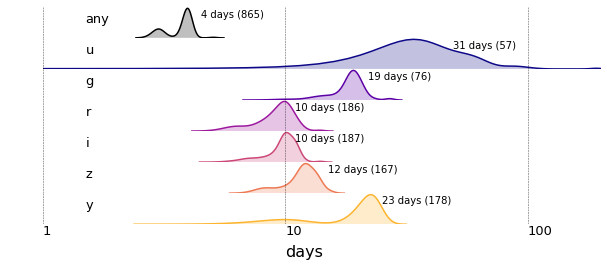
\includegraphics[scale=0.7]{figures/intranight_gap.png}
\caption{Distribution of time gaps between observations for 75 simulations of the Rubin LSST Wide Fast Deep (for observations not in the same night,  healpix with 64 sides, roughly corresponding to 55 arcminute resolution). The top plot shows the distribution of gaps between observations of the same filed in \emph{any} filter, the following plots show the time gaps between observations in the same filter, as labelled. The plots are normalized and median gap value at the peak of each histogram across all \opsim s is indicated to the right of each distribution, along with the median  number of observations over the 10 year survey simulation. The distributions are smoothed with via Kernel density estimation algorithm. While all these \opsim s fulfill the requirements in the SRD \citep{lsstSRD} the distributions still show a significant range. See Section \ref{sec:intro}.}
\label{fig:tgaps_example}
\end{figure}
\end{center}
As measured by imaging surveys, astronomical objects are characterized by color, brightness, brightness ratio in different portions of the energy spectrum, position, shape, and the rate and direction of change in any of those features. This leads to a multidimensional phase space which can be explored. Different categories of phenomena lie in different regions of the phase space (see \autoref{fig:phasespace}). Accordingly, we identified the following features that can be measured in the Rubin Observatory data:
\begin{itemize}
\item Color
\item Time evolution
\item Motion    
\item Morphology
\item Association
\end{itemize}

We set morphology aside, as largely the power of the survey to measure morphological anomalies does not depend on the survey strategy, but rather on the image system design (e.g. resolution and depth). We assume that measuring anomalous associations depends on our accuracy in measuring the properties of each object.

Having identified features that can be extracted by the Rubin Observatory data, and the LSST in particular, such as color information or lightcurve evolution, we measure the completeness of the survey in a hypercube in the feature space as a model-independent measure of the power to detect unknown-unknown transients.  
To measure dynamical anomalies in a completely model-independent way proves to be more difficult. Consider objects in our own galaxy. Having measured the proper motion of an object in the sky, our ability to understand if it is anomalous depends on  our accuracy in the motion measurement, and our ability to associate that object to a known galactic component with known proper motion distribution, given its coordinates, color, and brightness. Thus to measure the ability to identify anomalous proper motions we consider the photometric accuracy and the time gap between observations of the same field. One final parameter that influences our ability to detect anomalies is the sky footprint. Trivially, a larger sky footprint will lead to a higher event rate for anomalies. If one wants to maximise the chance of detecting extragalactic anomalies then a larger footprint would be favorable, while the probability of detecting galactic anomalies will scale with density of objects in the sky.

Ultimately, we define a set of metrics that can simply be summed to generate a $FoM$ for unknown-unknowns:

\begin{equation}
   FoM = \sum_{i={c,s,\mu,A_\mathrm{sky}, d }} w_i ~\mathrm{MAF}_i
\end{equation}

where $c, ~s, \mu,~ A_\mathrm{sky}, ~d$ represent the color, lightcurve shape, proper motion, footprint, and sky density respectively, and $w$ are weights that can be assigned to favor the discovery of, for example, transients over non-evolving objects, or galactic over extragalactic transients. We refrain from assigning weights and we normalize each \texttt{MAF} to the best of our ability in a 0-1 range, so as to provide a ``neutral'' comparison of the existing LSST simulations.

\subsection{\opsim~ Data}
\question{We need to describe \texttt{baseline v1.4} and the families, and put a table with all the names and families.}


%********************results***********************************

%\section{Results}

%\subsection{Color}


\section{Color and time evolution}\label{sec:timegaps}

\begin{center}

\begin{figure}[t!]
\centering 
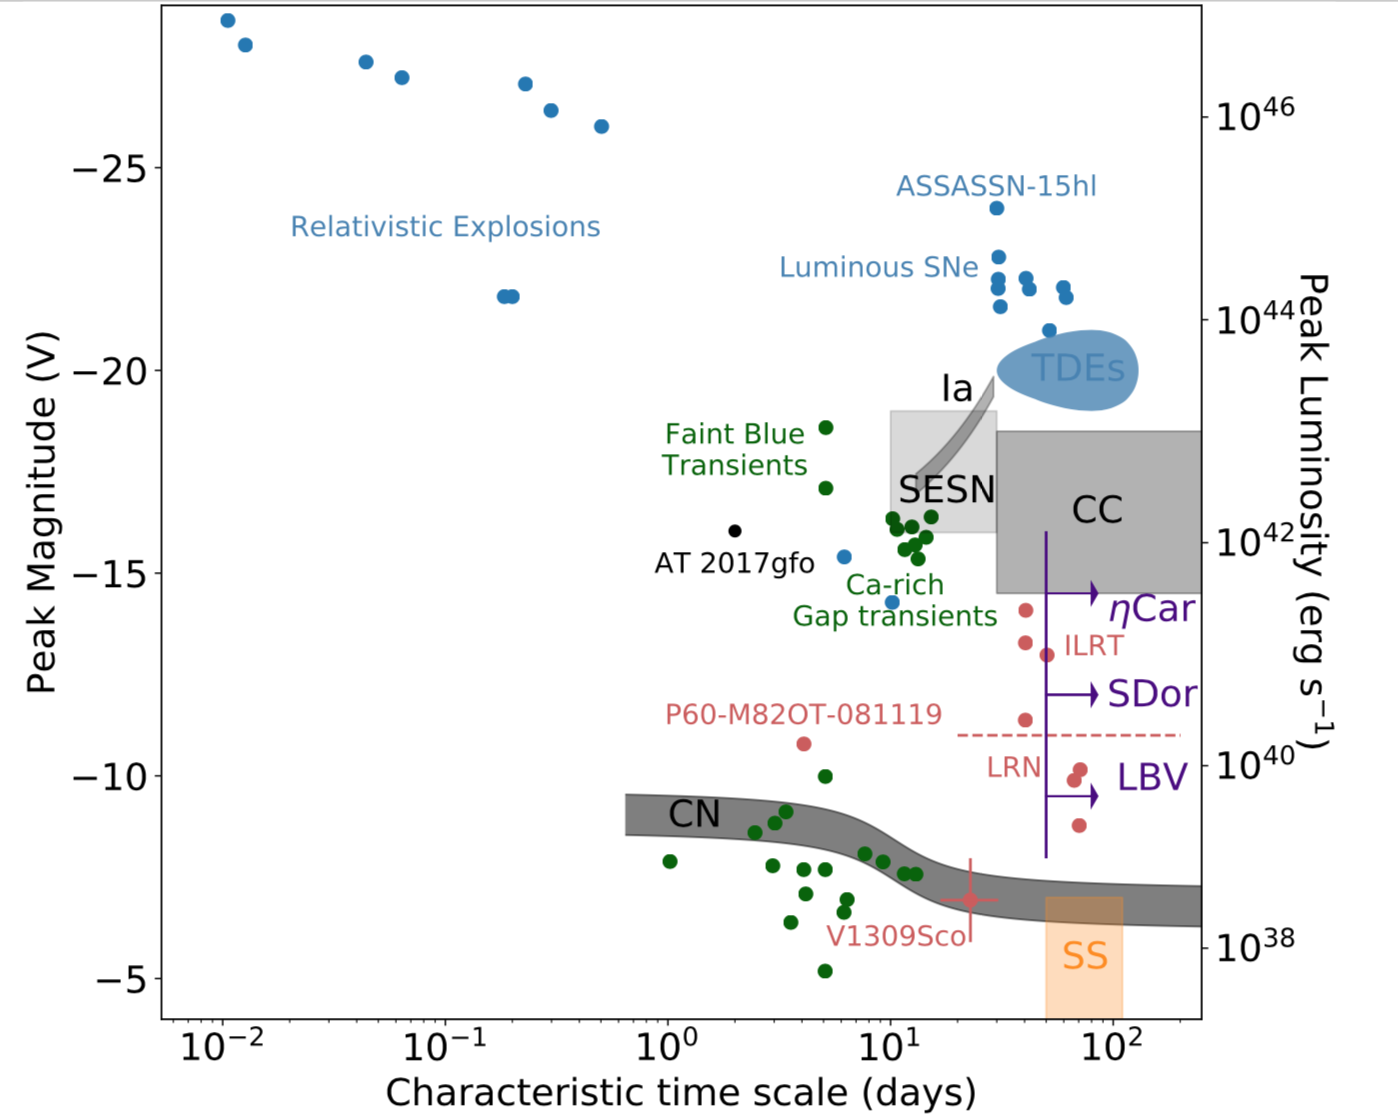
\includegraphics[scale=0.4]{figures/taumv_updated_wgap_lr.png}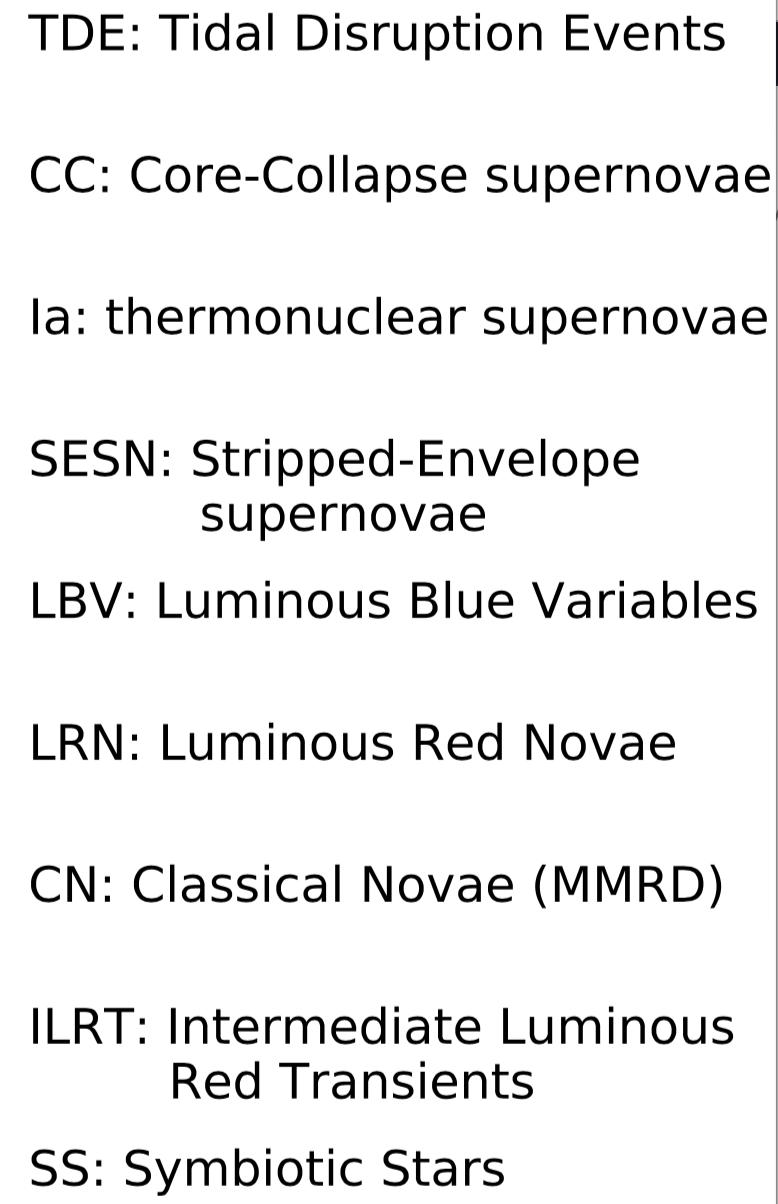
\includegraphics[scale=0.3]{figures/taumv_updated_legend.png}
\caption{The phase space of transients, reproduced with modifications and permission from \citet{lsst}: the intrinsic brightness is plotted against the characteristic time scale of evolution. Shaded areas indicate the  region of this phase-space occupied by various classes of objects and individual objects are indicated for some of the the less numerous classes. The notable gap at all intrinsic magnitudes fainter than -20 is likely due, at least in part, to an observational bias as surveys are typically not able to probe large volumes of the Universe at short time down to faint brightnesses. }
\label{fig:phasespace}
\end{figure}
\end{center}

Astrophysical transients and variable phenomenon captured humanity's curiosity through the history of science. Modern astrophysics and particularly the use of digital equipment in the last half-century enabled extremely fast paced advances in this field. Figure \ref{fig:phasespace}, reproduced from \citet{lsst}, shows the phase space of known astrophysical transients: transients and variable phenomena occupy different regions of this phase space of intrinsic brightness \emph{vs} characteristic time scales. At the beginning of the 20th century, essentially only supernovae were known to exist, and the phase space populated rapidly with many different classes of transients since then. It is worth noting the gap on the left of $\sim 1~\mathrm{day}$: while it is possible that this region is scarcely populated {\it intrinsically}, it is also true that an observational bias impairs discovery in this region:  to be effective in discovery and characterization surveys  need to reach high depth and high cadence simultaneously, while also surveying a large volume if phenomena in this region of the phase space are truly rare.




% time gaps distribution
\begin{figure}[t!]
\centering
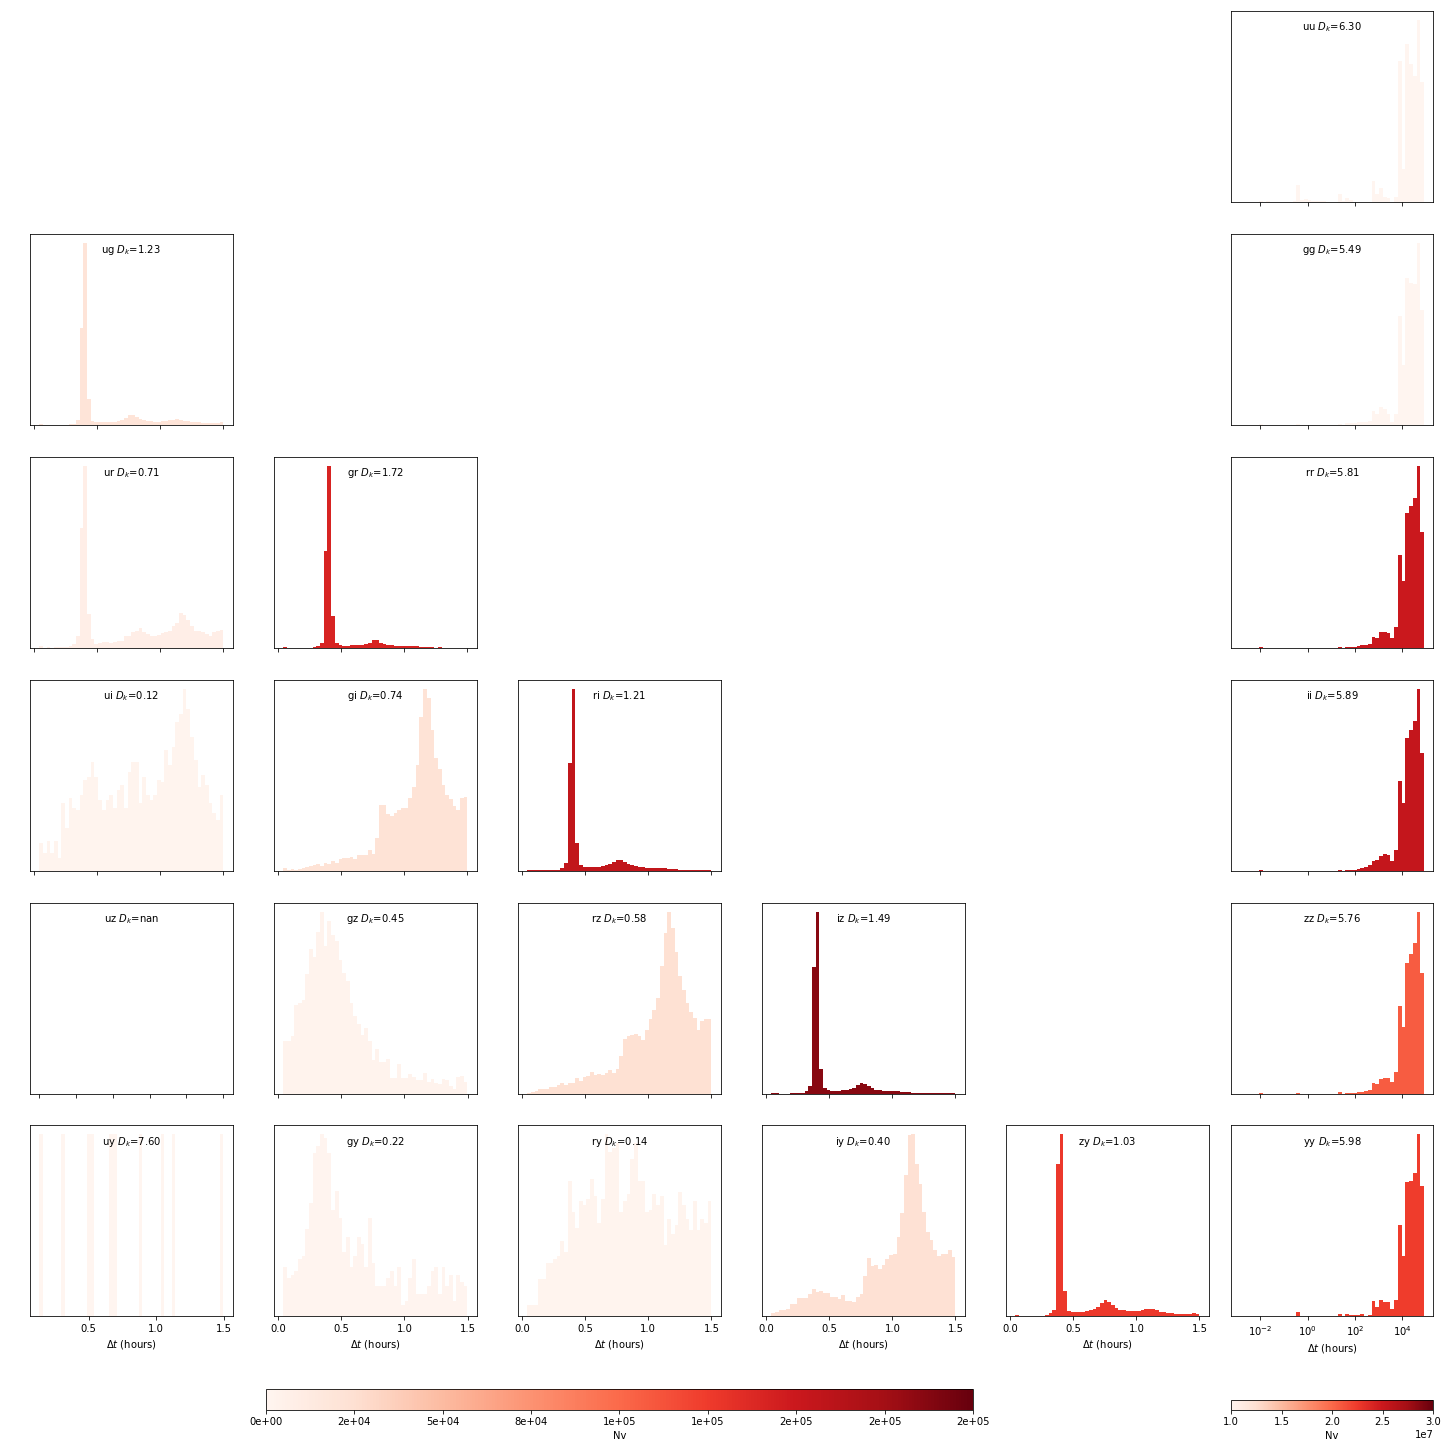
\includegraphics[scale=0.3]{figures/tgaps_hist.png}
\caption{
\new{The distribution of all time gaps for the \texttt{baseline v1.4} \opsim~ \question{Xiaolong please add the exact opsim name}. The triangle plot on the left shows all time gaps between different filters (which enable the measurement of color) within 1.5 hours. The column of plots on the right shows the distribution of time gaps in the same filter for the 10-year survey, which enables the measurement of brightness changes. The filters are indicated in each quadrant: from $u$ to $y$ moving from top to bottom and left to right. All histograms are normalized but the intensity of the color is proportional to the to total number of observations in that filter-pair, as indicated by the color bar. In each quadrant the value of $D_{KL}$ is  reported (see \autoref{sec:fom:tgaps}).  \question{We note that the majority of observations are taken with adjacent filters, which gives a narrow leverage on the spectral energy distribution (SED), and less power to measure color. Color is in fact better measured with filter that are more separated in wavelength, for example \emph{g-i} or \emph{r-z}, as described in \citep{Bianco_2019}}}
\question{Xiaolong: labels too small, color gets too faint, change label to $D_{KL}$}}
\label{fig:tGapshist}
\end{figure}

Due to their diversity in time scales, color, and evolution, the study of transients and particularly studies that aspire to discover new transient phenomena, requires dense space \emph{and} time coverage.  
%\question{Sufficiently high astrometric accuracy is also highly desirable in order to identify objects of interest with known (or unknown!) populations. I STILL DONT GET IT}. 
The LSST has both high photometric sensitivity and a large footprint, enabling the surveying of  a large volume of Universe. This provide us tremendous opportunities to study the variable sky. %: if the temporal cadence, then, is adequate \citep{lsstSB}, faint, rare and exotic objects are likely to be discovered. 
The LSST's capability to discover unknown-unknowns transients then largely depend on its observation cadence.

Different phenomena will benefit form different observation strategies because of the different phenomenological expression of their intrinsic physics. To make sure the observation strategies under design maximize  our chances to discover unknown unknowns, we created the {\it filterTGapsMetric}, which evaluates specifically  the ability of LSST's observation strategies to capture information about color and its time evolution at multiple time scales. 


\subsection{The \texttt{filterTGapsMetric}}\label{sec:fom:tgaps}

Rubin LSST will image the sky in six filter bands {\it u, g, r, i, z, y}. The {\it filterTGapsMetric} measures all time gaps between two filters in an \opsim, i.e, {\it ug, gr, ri} and so on. The \texttt{ filterTGapsMetric} Figure of Merit evaluates the coverage of time gaps for each filter-pair. We prefer an observation strategy that minimizes uncovered gaps, allowing the preference to differ for single-filter and for two-filter pairs. For example, assume one object changes its overall brightness across the spectrum within 3 hours. If we do not measure its brightness in at least two filters within this time we will not know what the true color of the object is. Homogeneous coverage within 1.5 hours in 2 filters maximizes our ability to measure color and color changes. Meanwhile, to detect brightness changes at different time scales we would prefer a distribution of time gaps for images in the same filter to be homogeneous in log-space.
%its color from {\it u} to {\it r} within 2 hours, if our cadence has no visits between {\it ur} within this time range, then we will definitely miss this kind of objects. 
%NOTE: this is not exactly how it works: we want the colors measured within 1.5 hours because slower would mean you cant tell if you observe color or lightcurve change. Within 1.5 hours we consider that we are agnostic about when to measure the color, and then diversifying within that range gives us less bias. We need to think about how to write this}

%\new{Following the naming convention of the COSEP, the map of evaluated quantities on a field-by-field basis is called the ``metric'', with the $FoM$ the result of the combination of the metric and any other weightings we impose, over the entire sky to distill the metric into a single scalar.}
%\question{this is described in the erlier section already} 
On a field-by-field basis, for each filter pair, the metric and $FoM$ are evaluated as follows:

\begin{itemize}
    \item select the survey (\emph{e.g.} WFD in this paper) and the observation time range using {\tt sqlconstraint} and slice the sky with HealpixelSlicer (see \autoref{sec:MAF}); 
    \item fetch observation times for each field for all visit in either of the two filters;
    \item perform a element-wise subtraction to get all time gaps;
\end{itemize}
\autoref{fig:tGaps} shows the distribution of time gaps for all filters pairs for the \texttt{baseline v1.4  OpSim} \question{Xiaolong please add the exact opsim name}. 


% KL divergence from uniform
\begin{figure}[t!]
\centering
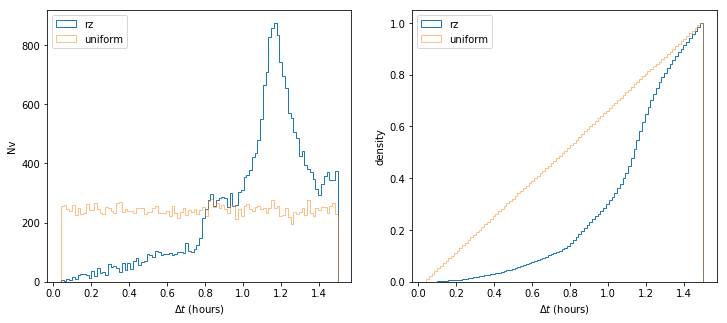
\includegraphics[scale=0.5]{figures/dkl_rz.png}
\caption{
Time gaps in $r-z$ (left) and $??$ (right) from the first year \question{Xiaolong fix the name: baseline operation v1.4} compared to the ``ideal'' distribution, plotted in orange: a uniform distribution for the colors (left) and a uniform distribution in log space for the lightcurve shape (right).  \question{This is not the right plot: we should have $g-i$ on the left and $g-g$ on the right in log scale; labels still too small }}
\label{fig:tGaps}
\end{figure}

% FOM from time gaps
 \begin{figure}[!th]
 \centering
 \gridline{
  \fig{figures/tgapsFOM_0.png}{0.4\textwidth}{(a)} 
  \fig{figures/tgapsFOM_1.png}{0.4\textwidth}{ (b)} 
  }
\caption{Figures of merit ($FoM$) for  75 \opsim~ runs based on the distribution of time gaps. The $FoM$ is calculated as described in Equation \ref{eq:fom:tgaps}. The plot on the \emph{left} shows the $FoM$ for repeat visits in the same filter.  The plot on the \emph{right} shows the value for observations in pairs of different filters. Each \opsim~ is presented as a bar whose length corresponds to the value of the $FoM$. For each \opsim~ FOMs for different filters are concatenated horizontally. For example: on the left the different color bars represent the time gap $FoM$ for different filters from $u$ to $y$  and the \opsim s are sorted by the total $FoM$, i.e. the sum of the FOMs, for that ``diagnostic''.  See Section \ref{sec:fom:tgaps}.  \question{When replaced with Sankey figure, update the caption to indicate changes are shown? FED: I think we should show the first figure of this set (now fig 4) in the text, and then the total figure of all metrics in this style, but put all intermediate ones in an appendix.}}
\label{fig:tgapsFOM}
\end{figure}
Armed with field-by-field time-gap distributions, the $FoM$ for the entire candidate survey strategy is then computed by measuring how well the distribution of time gaps matches our ideal distribution. 
\new{We use the Kullback-Leibler (KL) divergence (or relative entropy)~\cite{kullback1951} to measure the discrepancy between the ideal and observed distribution. The KL divergence provides an information-criteria based measure of the difference between two  distributions: the KL divergence from $Q$ to $P$ is defined as $D_{KL}(P||Q) = \sum P {\rm log}(\frac{P}{Q}) $. The KL divergence is not a distance, in the sense that it does not satisfy the triangle inequality, its not symmetric, and it is not normalized. To derive a normalized quantity from $D_{KL} $ we use $ e^{-D_{KL}} $, where two identical distributions, with  $D_{KL} = 0$  would contribute 1 to the sum, while $D_{KL} > 0$  would contribute $<1$. Thus a larger $FoM$ indicated a preferable simulation. This $FoM$ is naturally normalized between 0 and 1 for each field.} \new{\citealt{Bianco_2019} show that color can be measured reliably even for rapid explosive transients within 1.5 hours. Of course this is not necessarily true for unknown phenomena, but we will use this as a fiducial time interval and take the ideal distribution to be a uniform distribution between 0 and 1.5 hours.}
To probe lightcurve shapes, instead, we want to measure evolution at all time scales: repeat observations in the same filter at different  $\Delta t$, covering small time gaps to recover information about rapidly varying transients, or rapid evolution phases of transients, but also large time gaps to cover long time scales. We measure how similar a distribution of $\Delta t$  is to a logarithmic distribution by measuring $e^{-D_{KL}}$ between the observed distribution and a uniform distribution in $\log_{\rm 10}(\Delta t)$ for the entire 10-year survey.



The steps of the $FoM$ calculation then are:

\begin{itemize}
   
    \item compute the discrepancy-measure $e^{-D_{KL}}$ between the distribution of time gaps and an ``ideal'' distribution, for each filter-pair;
    \item Sum the discrepancy-measures over the filter-pairs, weighted by the \question{number of visit-pairs over the whole sky in each filter-pair} $N_k$, and by a ``scientific'' weight-factor $w$~that allows certain filter-pairs to be (de)-emphasized. This weighted sum is the $FoM$ for the OpSim of interest.
%    \item calculate figure of merit based the distribution.
\end{itemize}

The process is summarized in the relation:
\begin{equation}
    FoM_\mathrm{tGaps} =\sum_i^N \sum_{k=ug, gr,...}\frac{w_{k,i}}{N_{k,i}} e^{-D_{KL,k,i}}
    \label{eq:fom:tgaps}
\end{equation}
where $0 \le w_k \le 1.0$, $N_k$ stands for the number of visits\question{, and the index $i$ runs through the \texttt{healpixels} (\autoref{sec:MAF}). As indicated earlier, we do not choose any weights: the value of $w_{k,i}$ is always set to 1 in our calculations. Some filters and filter combinations may well be more useful than others to discover anomalies. Trivially, the value of $w_{k}$ could be set by the limiting magnitude for the shallowest filter in a filter pair. } 


\subsection{Results}



% time gaps distribution
%\begin{figure}[b!]
%\centering
%\includegraphics[scale=0.3]{figures/tgaps_cdf.png}
%\caption{
%The  distribution of all possible time gaps between two filters compared with the ideal uniform distribution. Time gaps in this plots are from the first year baseline operation v1.4. The KL divergence $D_{KL}$ is labeled on top of each subplots. The larger is the $D_{KL}$, the more different from uniform distribution. Filter pairs, u-z and u-y are missed. }
%\label{fig:dkl}
%\end{figure}




%\documentclass[onecolumn, 10pt]{aastex63}
%\usepackage{graphicx}%Include figure files
\newcommand{\red}[1]{{\color{red} #1}}


%\begin{document}
\section{Proper Motion metric}


% FOM from footprint
Vera Rubin Observatory, with LSST, could conduct extensive observation of the Galaxy which can lead to the discovering of new Galactic objects and phenomena. However, the extent to which the Galactic plane will be observed within LSST is uncertain \question{refer here to the other paper?}. In addition to transients and variable, the survey may discover objects with unusual proper motion within our Galaxy, or peculiar kynematic structures, such as streams. We consider both cases in this section. 
To measure LSST's potential to discover new objects with peculiar motion, we use two approaches: we generate synthetic objects in a Monte Carlo simulation within a proper motion distribution unlike that of any known Galactic component, and we take an exemplary Galactic structure, Sagittarius A and make it fainter, and move it farther away to test the limits of different \opsim s. 

\subsection {Monte Carlo simulation of object with unusual kynematics}
We use a Monte Carlo simulation to estimate \new{LSST's ability to distinguish unusual proper motion distributions for}
 stars in different part of the sky, considering the kinematics features of the known stellar Galactic components, the bulge, 
the disk, and the stellar halo, as described in \citet{Binney2008}. 
Stars in the Galaxy have a characteristic color, luminosity, and proper motion \new{which relates to their position and probability of belonging to one of the known Galactic structures}. From the color, luminosity, and coordinates, the expected proper motion can be estimated. 

Our simulation generates the distribution of proper motion for an object of a given magnitude changing the distance, and we iterated the algorithm for all the magnitudes in the range $[15,28]$ mag in $g$ band. 

The algorithm proceeds as follows:

\begin{itemize}
    \item generation of a set of distances $\mathbf{d}$ for stars within a distance range $[0,120]$~kpc, according to the distance distribution in \citet{Binney2008};
    \item \question{MISSING assignment of each star to a galactic component according to the relative density of objects given the  distance; \question{MISSING the step where you assign the luminosity tho do you consider the magnitude in this assignment?}}
    \item random association of a position in the sky to each object we simulate according the Maxwell-Boltzmann distribution for a star in  bulge, in the disk or in the halo; \question{MISSING the step where you assign the luminosity tho do you consider the magnitude in this assignment?}
    \item draw from the velocity distribution of the component the velocity of the object (see \autoref{MB_par});
    \item from the velocity components we calculate the tangential velocity, which represents the projection of the velocity vector on the sky plane;
    \item we calculate the simulated value of the proper motion as:
    \begin{equation}\label{PM_eq}
        \mu=\frac{v_{tan}}{d~4.74}  \arcsec/yr;
    \end{equation}
\end{itemize}



The velocity distribution of the \emph{known}-objects is parametrized according to a Maxwell-Boltzmann distribution (\autoref{MB_par}), while for the \emph{unusual}-objects we propose uniform velocity distribution in the range $\left[-5000,5000\right]$ $km/s$ to mimic a different group of stars that are moving in the same dynamic structure. \question{While this is not a non-parametric model, the uniform distribution is minimally informative (is it true???)}. 

\sout{Iterating the procedure over the number of objects we want to fill the survey with, we are able to build a distribution for the \emph{usual} and \emph{unusual} objects and comparing the two} \new{not really what you do: you create distributions, not objects one by one}


From the simulation we estimate the proper motion through  \autoref{PM_eq}, \new{we calculate the observed} distance as $d=10^{(0.20*M_r+1)}$, and measure the time gap between two consecutive observations of the field \question{in the same filter? only in g right - and why consecutive observations?}. 

With this we can estimate the proper motion $\mu$, and check if it can be measured by the survey: we assume that the proper motion has to be greater of the $5\%$ of the point-spread-function (PSF) full width half maximum (FWHM) to detect the motion. \new{In order to do this we leverage a series of MAF functions: we use the time gaps metric described in \autoref{sec:timegaps}, we extract the PSF from the \opsim~ catalog, as well as the signal-to-noise ratio $\frac{S}{N}$ of the measurement of a given star, obtained from the magnitude limit for the observation which is reported in the \opsim.}



\begin{table}
\centering
\caption{\label{MB_par}The table shows the values of the parameters for the three dimensional Maxwell-Boltzmann distribution. Considering the the Galactic coordinate system, the velocity spread in the table represents a three component vector which element are its radial, transverse and axial component respectively. The form of the distribution consider also the effect from the asymmetric drift, $v_a$. $n_0$ is the normalization factor.}
\begin{tabular}{|c|c|c|c|}\hline
$f_{DF}=\frac{n_0}{(2\pi \sigma_v^2)^{3/2}}exp[-\frac{(v-v_a)^2}{\sigma_v^2}]$& $n_0$ &$v_a$[km/s] &$\sigma_v $[km/s]  \\\hline \hline
 Bulge & $0.02$ &100 & [120,95,75]  \\ \hline
 Disk & $0.98$ &10 & [40,30,20] \\ \hline
 Halo & $0.05$ &200 & [130,105,85]\\ \hline
\end{tabular}
\end{table}

The simulation let us analyse how the distribution of objects \question{SHOULD BE MORE CLEAR from a different physical background} will be observed with a given observing strategy. To understand which strategy will perform better in detecting unusual objects we measure what  fraction of unusual objects are in fact classified as unusual. To classify the object as known or unusual we use the Likelihood ratio and measure the likelihood of an object with a given set of observables  $\theta$ to belongs to the known distribution with parameters $\theta_0$ or to an unknown distribution:

\sout{which tracks the gradient of the likelihood function respect a given parameter vector }\question{dont know what tracks the gradient mean:}

\begin{equation}
    S\equiv Log\left(\frac{\mathcal{L}(\theta)}{\mathcal{L}(\theta_0)}\right),
\end{equation}
where $\mathcal{L}$ is the likelihood function, $\theta$ is the parameter vector of the object and $\theta_0$ is the parameter array for a normal distributed object in the proper motion space.

The Likelihood function is described as follow:
\begin{equation}
    \mathcal{L}\left(\mu_i|\mathbf{X}, mag, \Delta t\right)=\frac{\phi_c(\mathbf{X}_i)}{\phi(\mathbf{X}_i)} f_{DF}\left(\mathbf{v}\right)P\left(\mu|mag, \Delta t\right),
\end{equation}
where the first term of the product is the membership probability of the object to the disk, the bulge or the halo of the Galaxy, $f_{DF}\left(\mathbf{v}\right)$  is the velocity probability distribution, $P\left(\mu|mag, \Delta t\right)$ is the probability to see an object moving in a given time interval with a magnitude over the detectability threshold for a proper motion distribution.
As it had been highlighted in \citet{Kuijken02} the uncertainties on the position due to the magnitude of a moving star can be estimated as: $\sigma_{\Delta x}= \frac{S}{N}*0.67* FWHM$; since the uncertainties on the time is negligible,  $\sigma_{\Delta x}$ is the main contribution on the measurement errors, thus the probability $P\left(\mu|mag, \Delta t\right)$ can be derived as:
\begin{equation}
    P\left(\mu|mag, \Delta t\right) \approx e^{-\frac{(0.05*FWHM-\Delta t *\mu)^2 }{(0.67*FWHM)^2}*(\frac{S}{N})^2},
\end{equation}
where the term $0.05*FWHM$ is the space gap threshold for a motion to be detected, $\mu$ is the simulated proper motion, $\frac{S}{N}$ is the signal to noise ratio and $\Delta t$ is the survey duration.

\begin{figure}
\centering
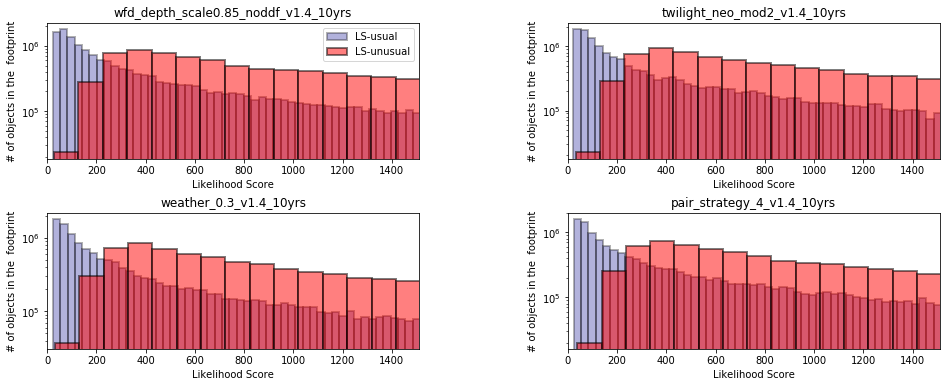
\includegraphics[scale=0.55]{figures/LS_distribution.png}
\caption{The Likelihood score distribution of simulated known and kynematically unusual objects as observed by four different \opsim s.  \question{FED: not sure what the next sentence means }. The trend of unusual object grows as the number of usual detected objects decrease. \sout{The area of the not overlapping region is related to the fraction of unusual objects detectable within the specific observation strategy, thus it is a good tracer of the \opsim~ skills.} \new{The figure of merit we define is the area of the histogram of unusual objects that is does not intersect the histogram of known objects (appropriately normalized). }}
\label{fig:PM_distribution}
\end{figure}
The Likelihood $\mathcal{L}\left(\mu_i|\mathbf{X}, mag, \Delta t\right)$, \sout{with the underlined contribution},  was used in the likelihood score estimation to track the known and unusual objects distributions, thus giving an hint on how good  a specific observation strategy is at detecting unusual observations.

\begin{figure}
\centering
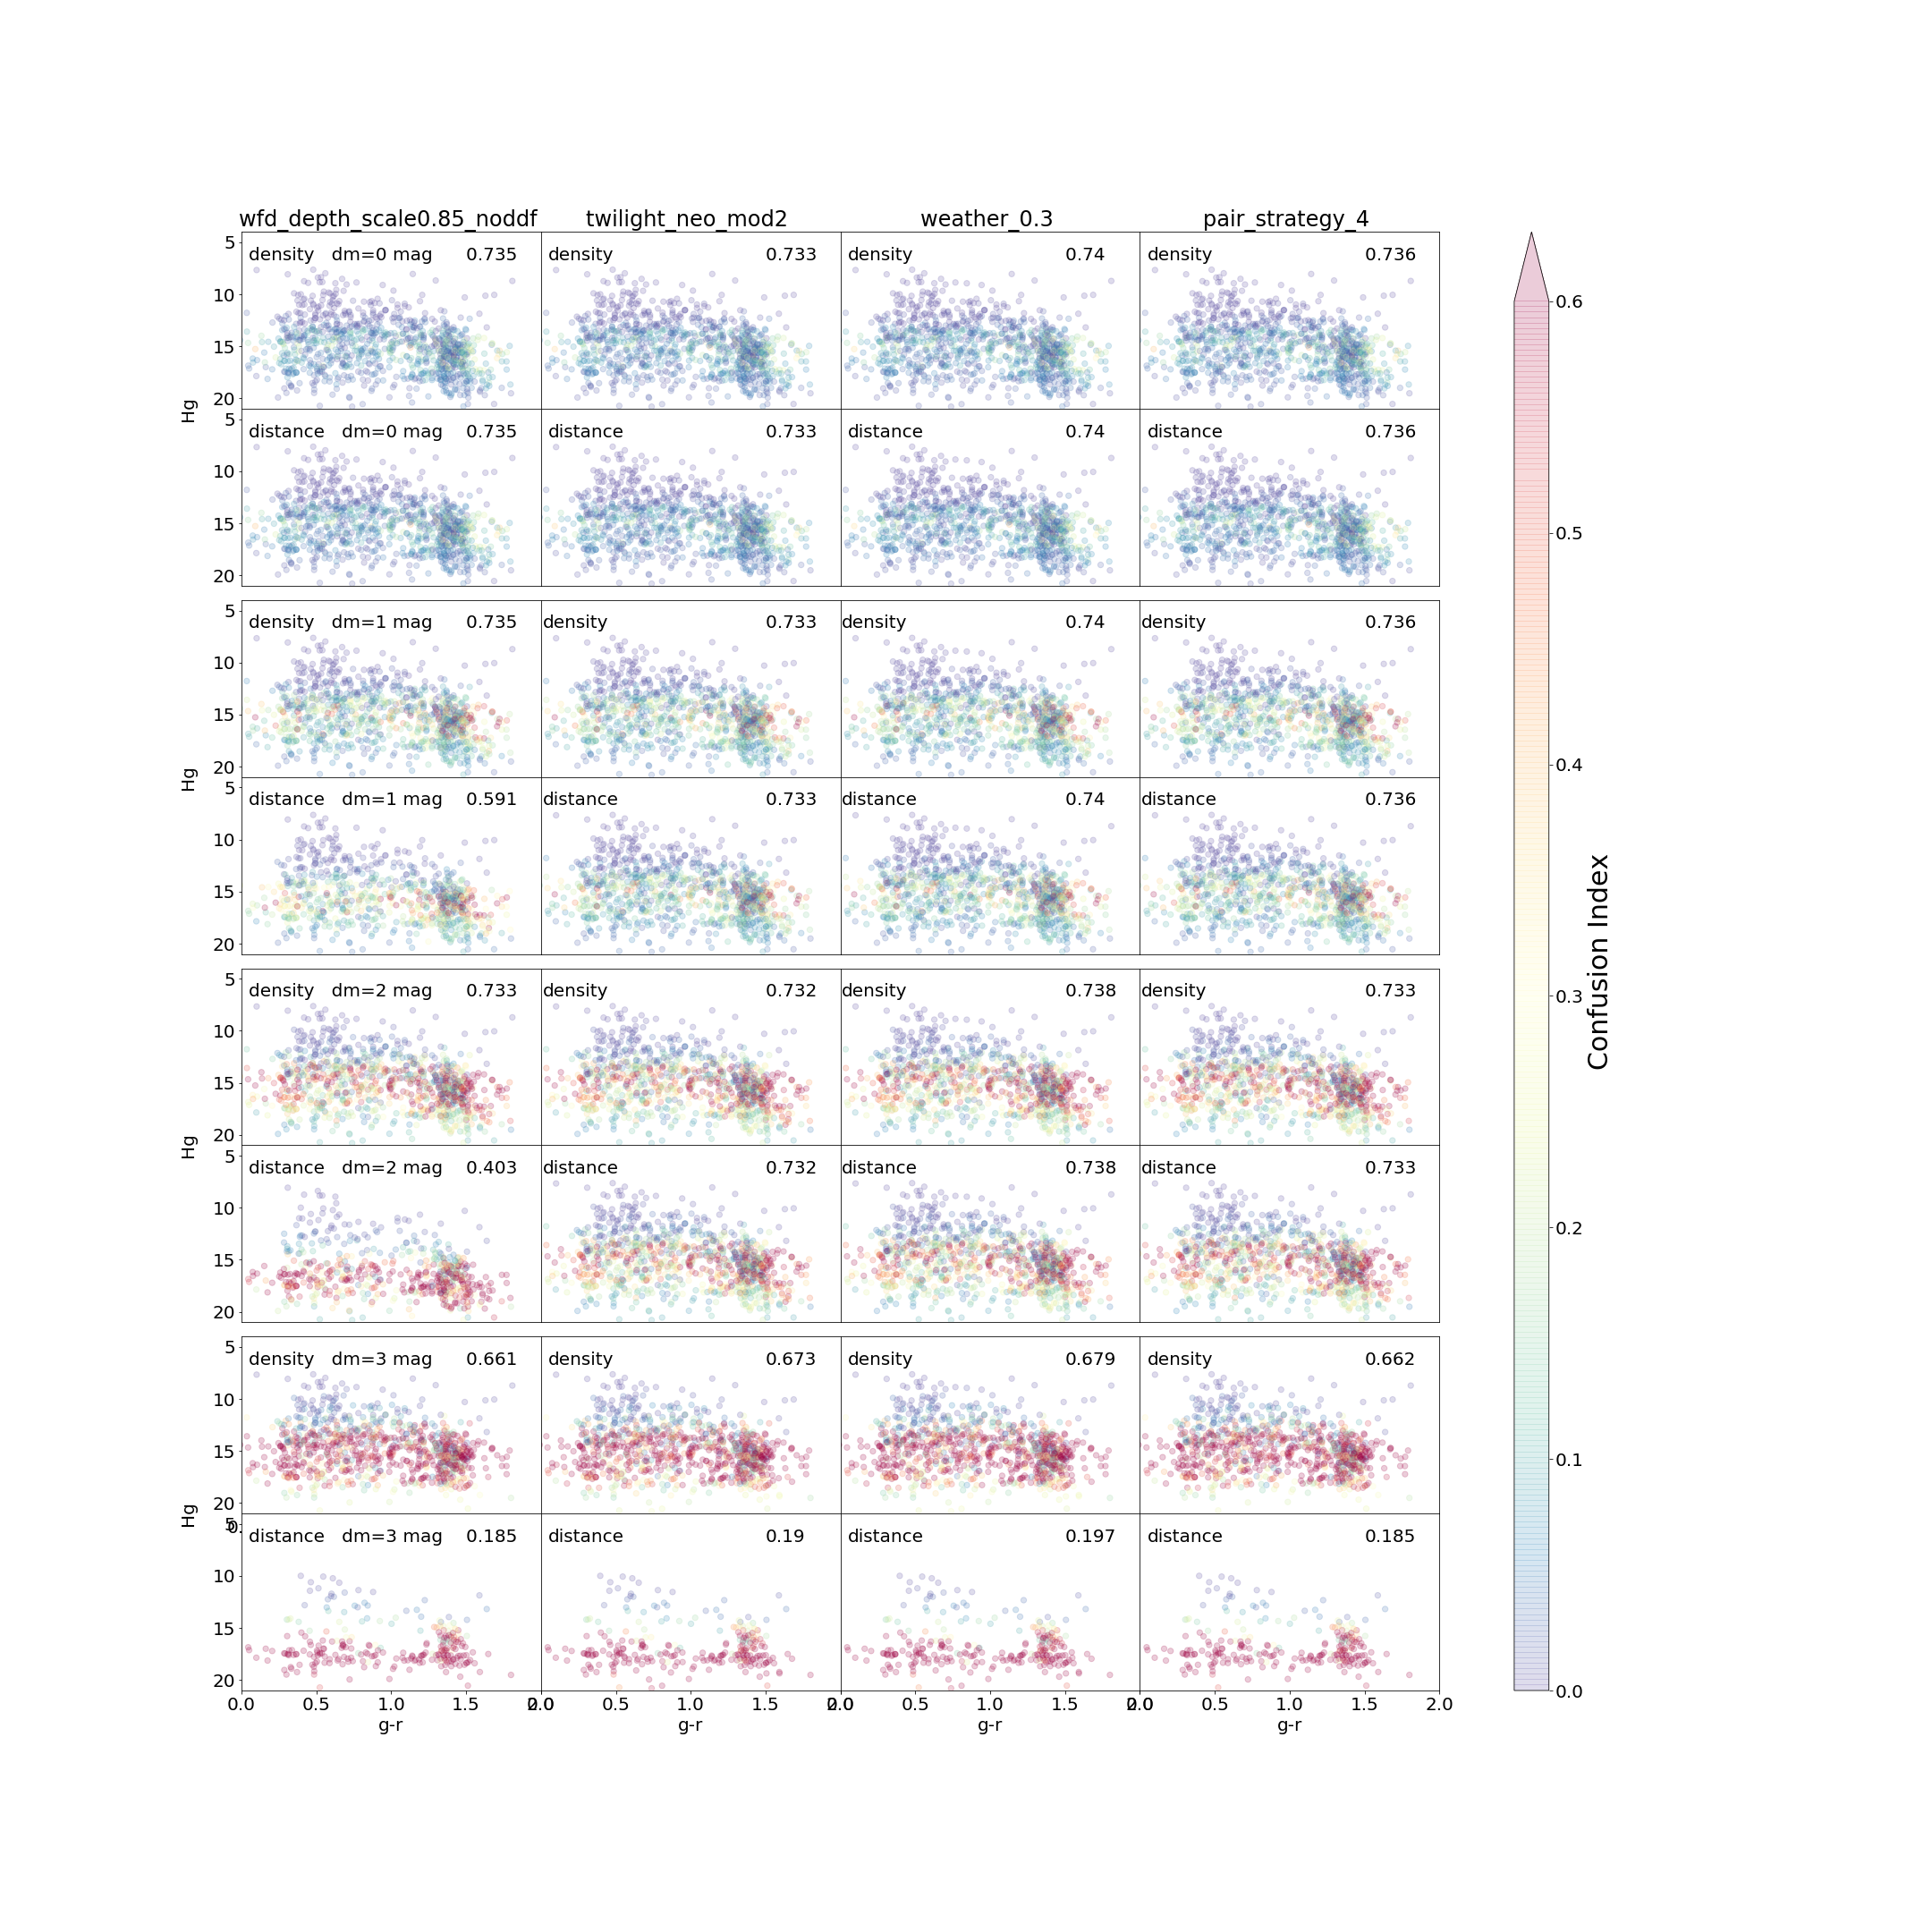
\includegraphics[scale=0.28]{figures/ConfunsionIndex_10yrs.png}
%\vspace{-20mm}
\caption{The figure presents the outcomes of the analysis on the 10 yrs survey for four different Opsims, and it shows the ability on reproducing the Proper Motion Diagram (PMD) in \citet{Carlin12} considering two possibilities: changing distance or density of Sgr. From the top to the bottom of the figure we have increased the magnitude to simulate either more distant or denser stellar structures then Sgr, the specific mode of the simulation is expressed in the top left of the plots. When we simulated changing in distance we considered related changes for the PM, following $\mu_{new}=\frac{\mu_{old}}{10^{\frac{\Delta m}{5}}}$. Looking at the top right in the plots there is shown the fraction of detected stars; we noted that  changing the distance of about $\Delta m= 3$, we already lose more than $50\%$ of the precision in detecting the proper motion and we are able to detect just about the $20\%$ of the stars in the sample. \question{remove y labels from all but the first column, put space between every 2 rows (sets of density and distance)}}
\label{fig:Conf_Idx}
\end{figure}

\subsection{Sagitarius A simulations}

\sout{ To verify the ability to support these expectations, w}

We used the Sagitarius A structure as toy model to analyze the ability of an \opsim~ to discover streams. In order to give a description on the performance of the different strategies, we reproduced the analysis from \citealt{Carlin12} on the proper motion of the \question{Sagitarius (Sgr) trail tidal debris} \sout{, using the same data set used in the cited paper (see Fig. \ref{fig:Conf_Idx}), to analyze how the science is improved in using one strategy respect another,} and we as two questions: if the stream were fainter could we still detect it? and could we detect it were farther away? To answer these questions we (1) decrease the magnitude of all stars in the dataset used in \citet{Carlin12} figure 10. This can be interpreted as probing if the same stream could be detected using main sequence stars, instead of stars in the Giant branch. (2) decrease the magnitude \emph{and the proper motion} of all stars in the dataset used in \citealt{Carlin12}, which corresponds to move the stream farther away. We measure:

\begin{itemize}
    \item the fraction of detection we lose as they exceed the magnitude limit of the survey.
    \item the fraction of stars that cannot be detected without being confused with nearby stars, \ie~ detections that fall into an error ellipse: \emph{confusion index};
    
\end{itemize}

\sout{The toy model reproduced the same structure as Sgr in two different cases:  w} We moved Sgr A  within a distance range $[28,111]$ kpc , changing the proper motion of the sources accordingly to $\mu_{new}=\frac{\mu_{old}}{10^{\frac{\Delta m}{5}}}$; we dimmed it with the range $[0,3]$ mag, changing the density of Main Sequence stars, thus letting the structure get fainter \question{when you move it away do you move it away by the correct amount that corresponds to a magnitude drop of 0, 1, 2, 3?}. 

For all \opsim s, we note that, with reference to  \autoref{fig:Conf_Idx}, we rapidly reach the $50\%$ limit in the confusion index \question{need to explain this confusion index better}. This means that for structures dimmer than Sgr A by $2$ mag we \sout{would have less sensibility in measuring colors and proper motion} only be able to use 50\% of the stars in the stream. The analysis pointed out also that for a Sgr A-like structure farther away by $111$ kpc we will be able to detect only   $\sim20\%$ of the stellar objects. 
\question{But what is the metric??}


Another important aspect we stress is the ability of the different strategies in detecting objects that moves and for which it is possible to detect the motion itself. To do that we simulated light curves that go on and off during the survey duration such as the transients can be observed at least twice, and its motion can be detected as well. \question{need more on this}


\subsection{Figure of merit}
The metrics described are able to determine, from the astrometric point of view, the best strategy to detect the proper motion. Combining them with the footprint coverage we are able to underline if there are region of the Sky that are not visited too much or not visited at all, producing a bad performance rate of the observation strategy. 
The figure of merit for a survey is defined as:
\begin{equation}
    FOM = N\frac{\sum_i MAF_i\cdot w_i}{\sum_i w_i}
\end{equation}
where $N$ is a normalization factor and the $MAF_i$ is the outcome of the metric for the \emph{i}-th field, $w_i$ is a weighted factor. The weight used is the frequency of the MAF value overall the footprint.   


\begin{figure}
    \centering
    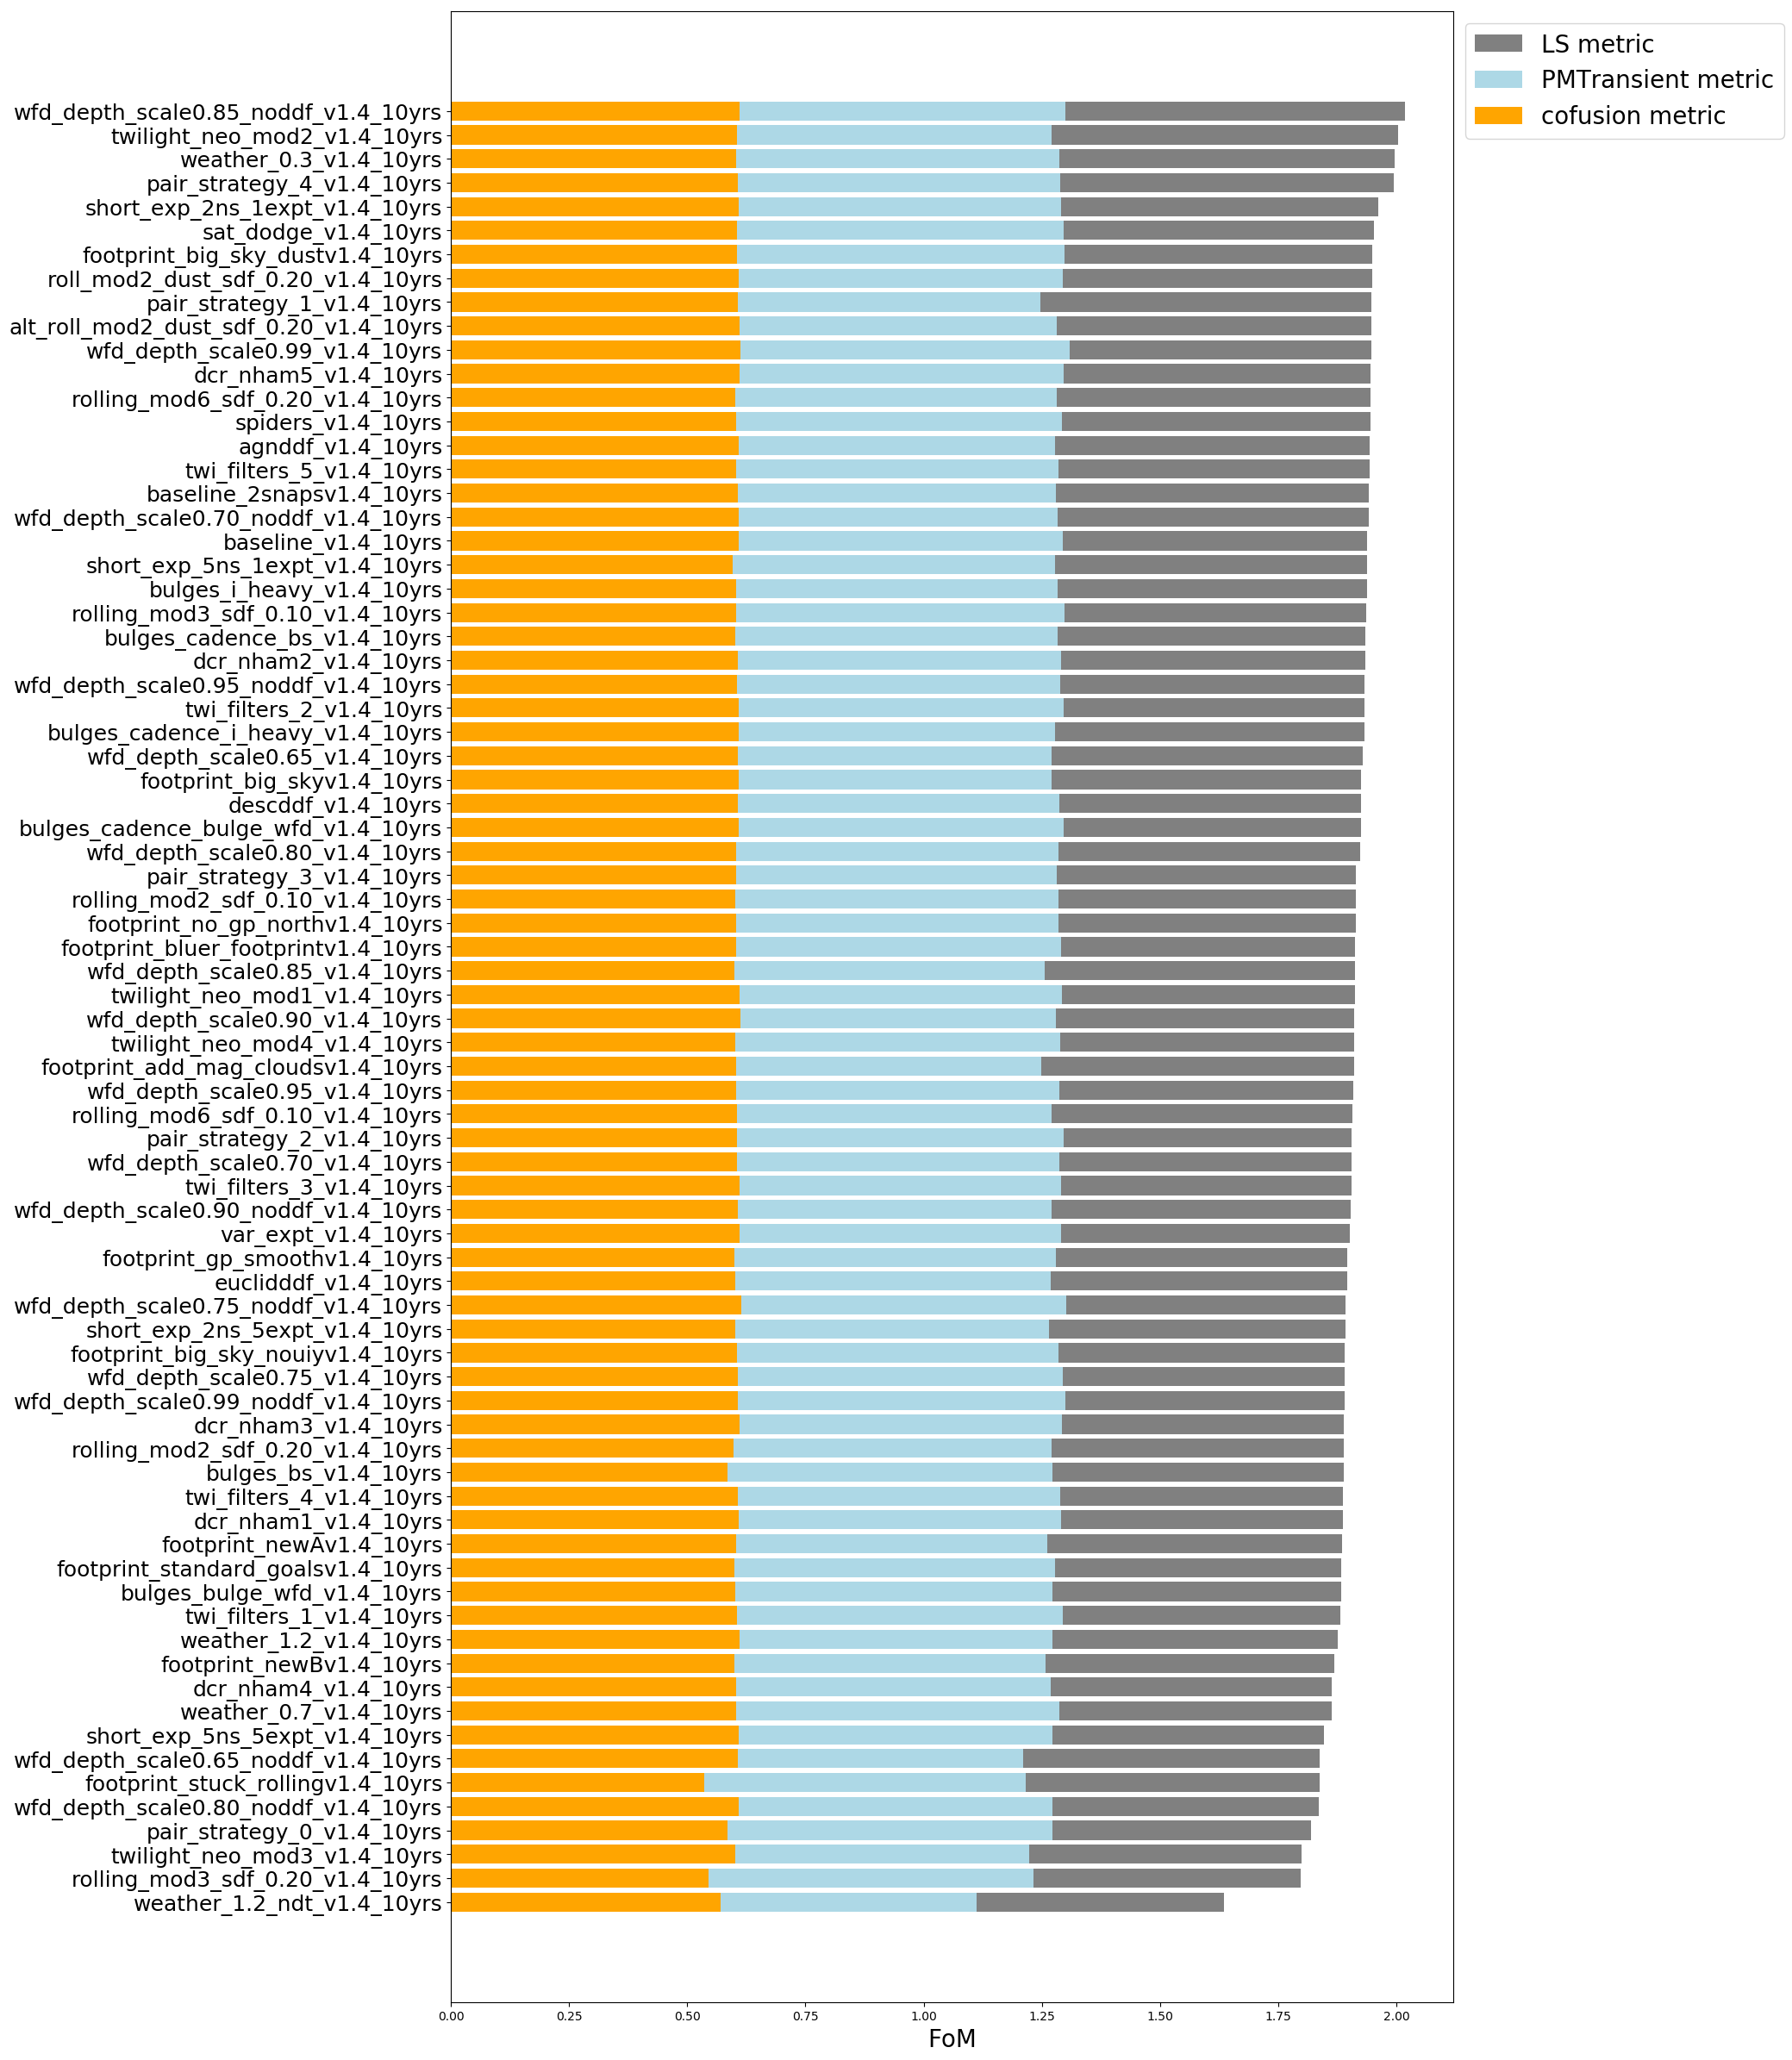
\includegraphics[scale=0.28]{figures/FOM_astrometry.png}
    \caption{}
    \label{fig:FOM_astrometry}
\end{figure}

\subsection{Results}

% \end{document}

\question{I propose we leave the footprint last since it is important for both time gaps and proper motion}
\begin{figure}
\centering
\gridline{
  \fig{figures/footprintFOM_0.png}{0.4\textwidth}{(a)} 
  \fig{figures/footprintFOM_1.png}{0.4\textwidth}{ (b)} 
}
\caption{The figure of merit $FoM_{Gal}$ for all 75 \opsim~ runs (for the WFD surveys) based on footprint coverage and star density as described in Section \ref{sec:fom:footprint } (expression \ref{eq:fom:footprint}). \new{Colors and symbols denote filter-combinations using the same conventions as in Figure \ref{fig:tgapsFOM}}. \question{the right plot is shrter than the left one...}}
\label{fig:starDensity_FOM}
\end{figure}



\section{Footprint}\label{sec:fom:footprint }
Footprint coverage is another important factor which play an crucial role in determining LSST's ability to discover anomalous and unusual phenomena.

We evaluate what fraction of the sky is covered by an observing strategy for each filter pair. Although an object may have an anomalous color which could be detected in a single visit pair, we focus here on transients and proper-motion and we want to observe a field repeatedly to detect changes. \question{This seems too demanding! maybe 1/2 that? would that not give enough differences?}. We use the median number of visits $N_{median}$ in \texttt{baseline v1.4} as the fiducial threshold: a field is considered well observed if it has more observations than the \question{$\frac{1}{2}N_{median}$}.  
To do this, we perform the follow steps for each field, 

\begin{itemize}
    \item count number of visits within 1.5 hours for each filter pair; 
    \item check if $N ~>~\frac{1}{2}N_{median}$;
    \item sum over all fields that pass requirement.
\end{itemize}

However, depending on whether a scientist's focus is on extragalactic or  galactic anomalies, the preferred footprint would be different: for extragalactic anomalies one would simply want to maximize the sky coverage, whereas for Galactic science the probability of discovering an anomalous object or phenomenon would scale with the number of objects in the Galaxy in that observing field. Therefore, in addition to the $FoM$ just described, which focuses on extragalactic science ($FoM_\mathrm{EG}$), we include one further footprint figure f merit ($FoM_\mathrm{Gal}$) that scales with the field's star density: this $FoM$ is the sum of each field that meets the requirements as described above, multiplied by the number of stars in that field.

These FoMs for an \opsim~ are therefore defined as: 
\begin{eqnarray}
    p_{i} &=& 1 ~\mathrm{if} ~N ~>~\frac{1}{2}N_{median} ~\mathrm{else}~ 0\\
    FoM_\mathrm{EG} &=& \sum_{i} p_{i}, \\
    FoM_\mathrm{Gal} &=& \sum_{i} s_{i} p_{i}.
\label{eq:fom:footprint}
\end{eqnarray}
where  $s_{i}$ is the star density (which is obtained from existing MAF functions) for the $i$th field, and $p$ equals to 1 or 0 depending on whether the field meet the minimum requirements. 

\question{2020-06-03 WIC - this subsection could be a little clearer: the text is a bit vague on how expressions \ref{eq:fom:tgaps} and \ref{eq:fom:footprint} relate to each other (e.g. the $N_i$~in expression \ref{eq:fom:footprint} is very much {\it not} the same thing as the $N$~in expression \ref{eq:fom:tgaps}). The text should make clear whether Figure \ref{fig:starDensity_FOM} refers to the {\it combined} Figure of merit (including both the tgaps and the density \& footprints) or just the density \& footprints.}

These $FoM$s of merit for all 75 simulations are plotted in Fig. \ref{fig:starDensity_FOM} and \question{Xiaolong add the figure here for the FOMEG}. 
%\subsection{Proper Motion}
\section{Conclusion and Discussion}



\begin{center}
\begin{figure}[t!]
\centering
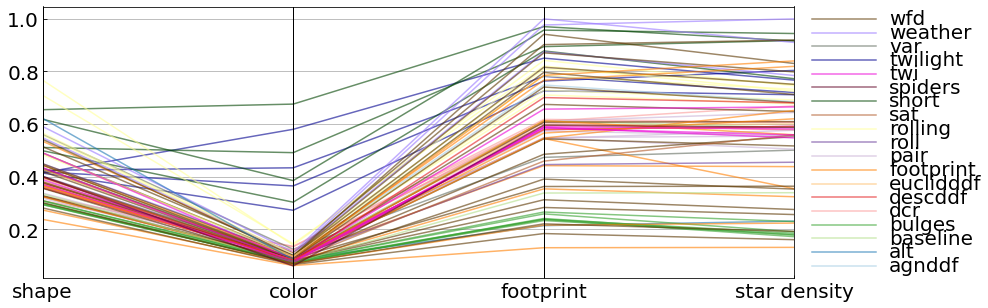
\includegraphics[scale=0.5
]{figures/opsimParallelCoord.png}

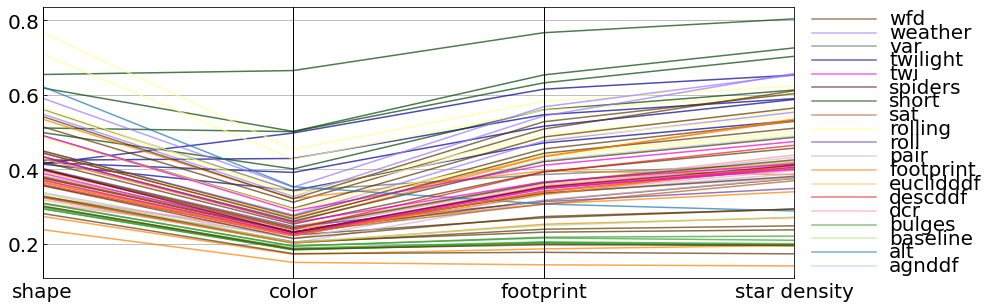
\includegraphics[scale=0.5]{figures/opsimParallelCoord_cum.png}
\caption{The result of the four$FoM$ for all available OpSims. Different FoMs are shown along the $x$ axis, as labeled, for all OpSims. Different families of OpSims are shown in different colors, as labled. On the top each$FoM$ is shown individually, at the bottom their cumulative sum (normalized) is shown. \question{which is better?} The ``color'' FoM, which measures how regularly time gaps are collected within 1.5 hours, generally leads to smaller values. While the \opsim~ switch places, they don't generally do so in  a very significant fashion. \question{which families are better?}}
\label{fig:opsimPC}
\end{figure}
\end{center}


\acknowledgments
We used the following packages:
\begin{itemize}
\item{\texttt{python}}
\item{\texttt{pandas}}
\item{the \texttt{glasbey} package to generate maximally separable colors. \citep{glasbey2007colour}}
\item{Webplot Digitizer \citep{digitizer}}
\end{itemize}
We thank 

% 2020-06-10 WIC - I recommend we use bibtex to handle the references, it's a lot less work than using bibitems (since unused references are not put in the article, the output is automatically sorted by alphabetical then date order, and the citations can be pasted from ADS' "Export Citation" link into the .bib file.). There is a github repo with a list of project publications at the following location:
% https://github.com/lsst-pst/LSSTreferences/
\bibliography{refs}

%
%********************references***********************************
%
%
%
%% 2020-06-10 - All of the entries below have been reproduced in the refs.bib file ,with the exception of the NSF portfolio review (for which I couldn't find a bibtex version)


\begin{thebibliography}{50}

\bibitem{sloan} Donald G. York et al. The Sloan Digital Sky Survey: Technical Summary. ApJ., 120, 1579-1587 (2000). 

\bibitem{2mass} Skrutskie, M.F., et al. 2006. The two micron all sky survey (2MASS). The Astronomical Journal, 131(2), p.1163 (2006).

\bibitem{lsst} Zeljko Ivezic et al. LSST: from Science Drives to Reference Design and Anticipated Data Products. ApJ., 873, 111, 44 (2019).

\bibitem{lsst_sb} LSST Science Collaboration. LSST Science Book, Version 2.0. {\it arXiv:0912.0201}. (2009).

\bibitem{nsf} National Science Foundation Division of Astronomical Sciences Portfolio Review Committee. Advancing Astronomy in the Coming Decade: Opportunities and Challenges. (2012).

\bibitem{spitzer} Michael W. Werner, et al. The Spitzer space telescope mission. The Astrophysical Journal Supplement Series 154.1. (2004).

\bibitem{decam} Brenna Flaugher, et al. The Dark Energy Camera. The Astronomical Journal 150.5:150. (2015).

\bibitem{altas} Robert Jedicke, et al. ATLAS: asteroid terrestrial-impact last alert system. AAS/Division for Planetary Sciences Meeting Abstracts. 44. Vol. 44. (2012).


\bibitem{lsst_gaia} 

\bibitem{obs_strategy}
\end{thebibliography}



\end{document}